\section{Ground station networks}

There are a lot of unknowns in this area. We don't know which network will be used, who will be participating or what kind of radio equipment participants will have. 

Some different possible networks are simulated using the same constraints as at Gløshaugen. The results are summarised in \autoref{tab:networks}.

\begin{figure}
\begin{subfigure}{.5\textwidth}
	\centering
	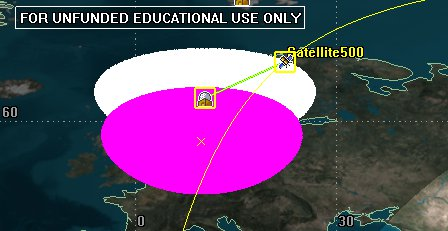
\includegraphics[width=\textwidth]{Figures/range_ntnu_aalborg}
	\label{fig:range_ntnu_aalborg}
\end{subfigure}
\begin{subfigure}{.5\textwidth}
	\centering
	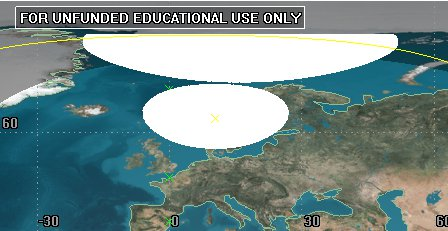
\includegraphics[width=\textwidth]{Figures/range_ntnu_svalbard}
	\label{fig:range_ntnu_unis}
\end{subfigure}
\begin{subfigure}{.5\textwidth}
	\centering
	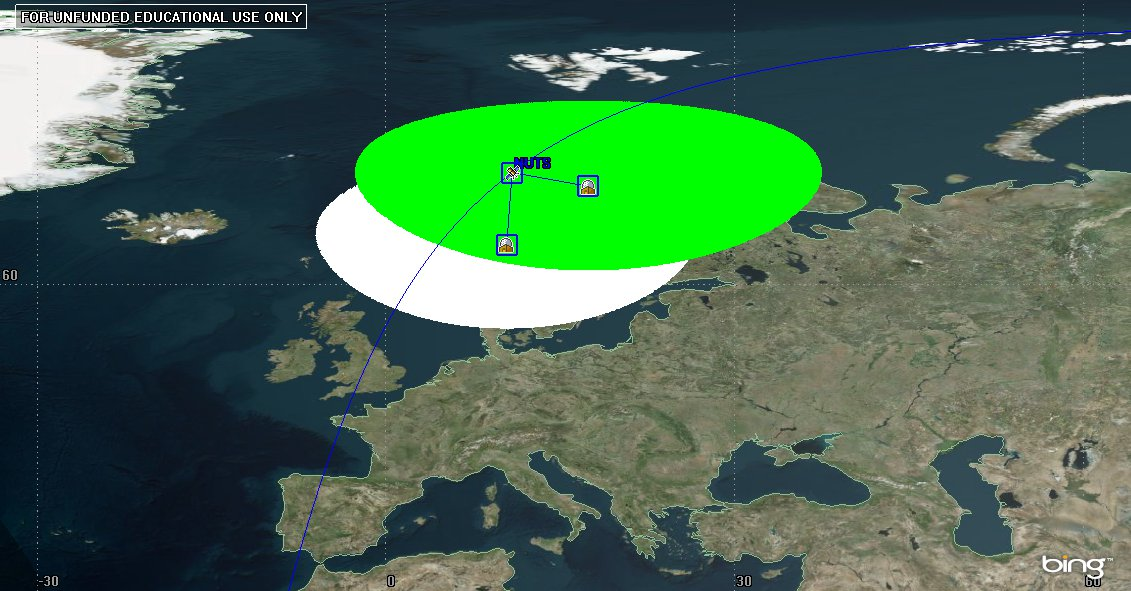
\includegraphics[width=\textwidth]{Figures/range_ntnu_narvik}
	\label{fig:range_ntnu_narvik}
\end{subfigure}
\begin{subfigure}{.5\textwidth}
	\centering
	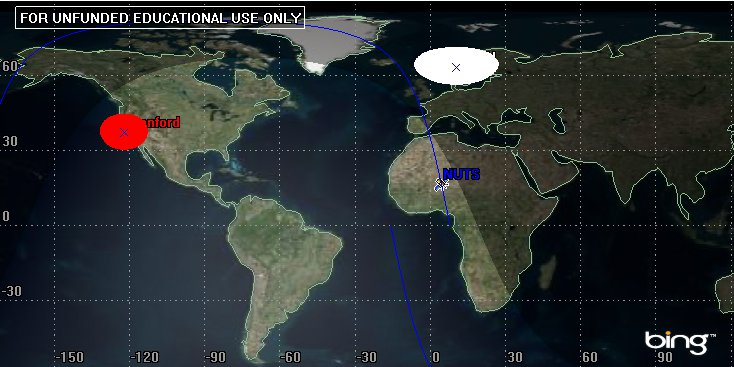
\includegraphics[width=\textwidth]{Figures/range_ntnu_stanford}
	\label{fig:range_ntnu_narvik}
\end{subfigure}
\caption{Some possible ground networks}
\label{fig:ground_networks}
\end{figure}

\begin{table}
	\begin{center}
	\begin{tabular}{l | c c}
  	Other locations & Time & Improvement \\
	\hline \hline
	Aalborg & 790s &  50\% \\
	\hline
	Longyearbyen & 1900s & 260\% \\
	\hline
	Narvik & 900s & 73\%  \\
	\hline
	Stanford & 800s & 54\% 
	\end{tabular}
	\end{center}
	\caption{Results of simulations}
	\label{tab:networks}
\end{table}

These results show that even cooperating with other norwegian/scandinavian universities will result in significant gains in download capacity, even though there will be a certain overlap in coverage. Cooperating with other universities further afield will also increase download capacity, but if they are located at lower latitudes the decreased number of passes observed will decrease their contribution.  


